\section{Depth Map Parameter Tuning}
\label{sec::52_dm}
Within this section, we shortly explore the effects of all tunable parameters on the depth map generation. Therefore, we utilize a simple experimental setup, which is shown in figure \ref{fig::52_wls_setup}.
\begin{figure}[h]
	\centering
	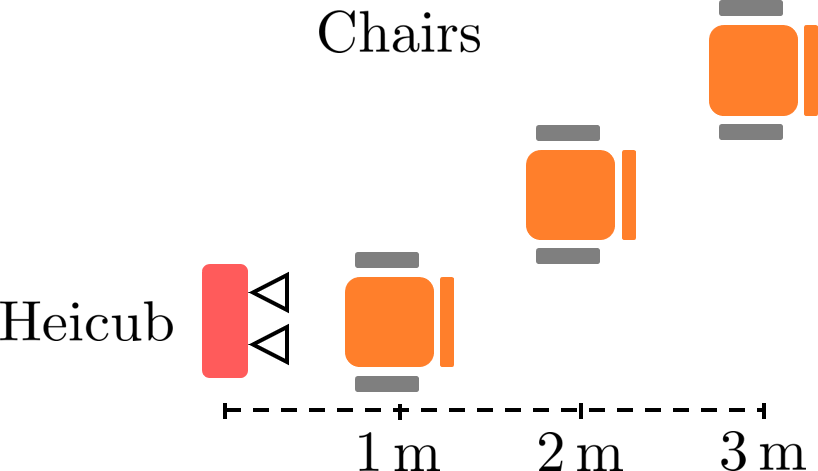
\includegraphics[scale=.4]{chapters/05_experiments/img/wls_setup.png}
	\caption{Setup for the parameter tuning of the depth map extraction. Heicub's cameras are indicated by the two triangles, of which you can find the view in figure \ref{fig::52_wls_rgb}}
	\label{fig::52_wls_setup}
\end{figure}
Within the setup, Heicub points its stereo camera towards three chairs that are located at a distance of $1\,\text{m}$ towards each other, and towards the cameras, so to cover close, medium, and far distances. The consecutive chairs are slightly shifted, in order to enable the simultaneous observation of all of them. The rectified view of the environment is shown in figure \ref{fig::52_wls_rgb}.
\begin{figure}[h]
	\centering
	\subcaptionbox{}%
	[.4\linewidth]{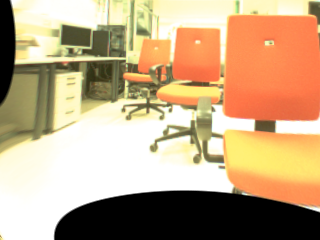
\includegraphics[scale=.3]{chapters/05_experiments/img/l_rgb.png}}
	\subcaptionbox{}%
	[.4\linewidth]{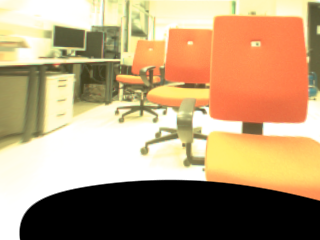
\includegraphics[scale=.3]{chapters/05_experiments/img/r_rgb.png}}
	\caption{Heicub's perspective of the scene for the setup in figure \ref{fig::52_wls_setup}. (a) shows the left camera's view, while (b) shows the right camera's view.}
	\label{fig::52_wls_rgb}
\end{figure}

\begin{figure}[h]
	\centering
	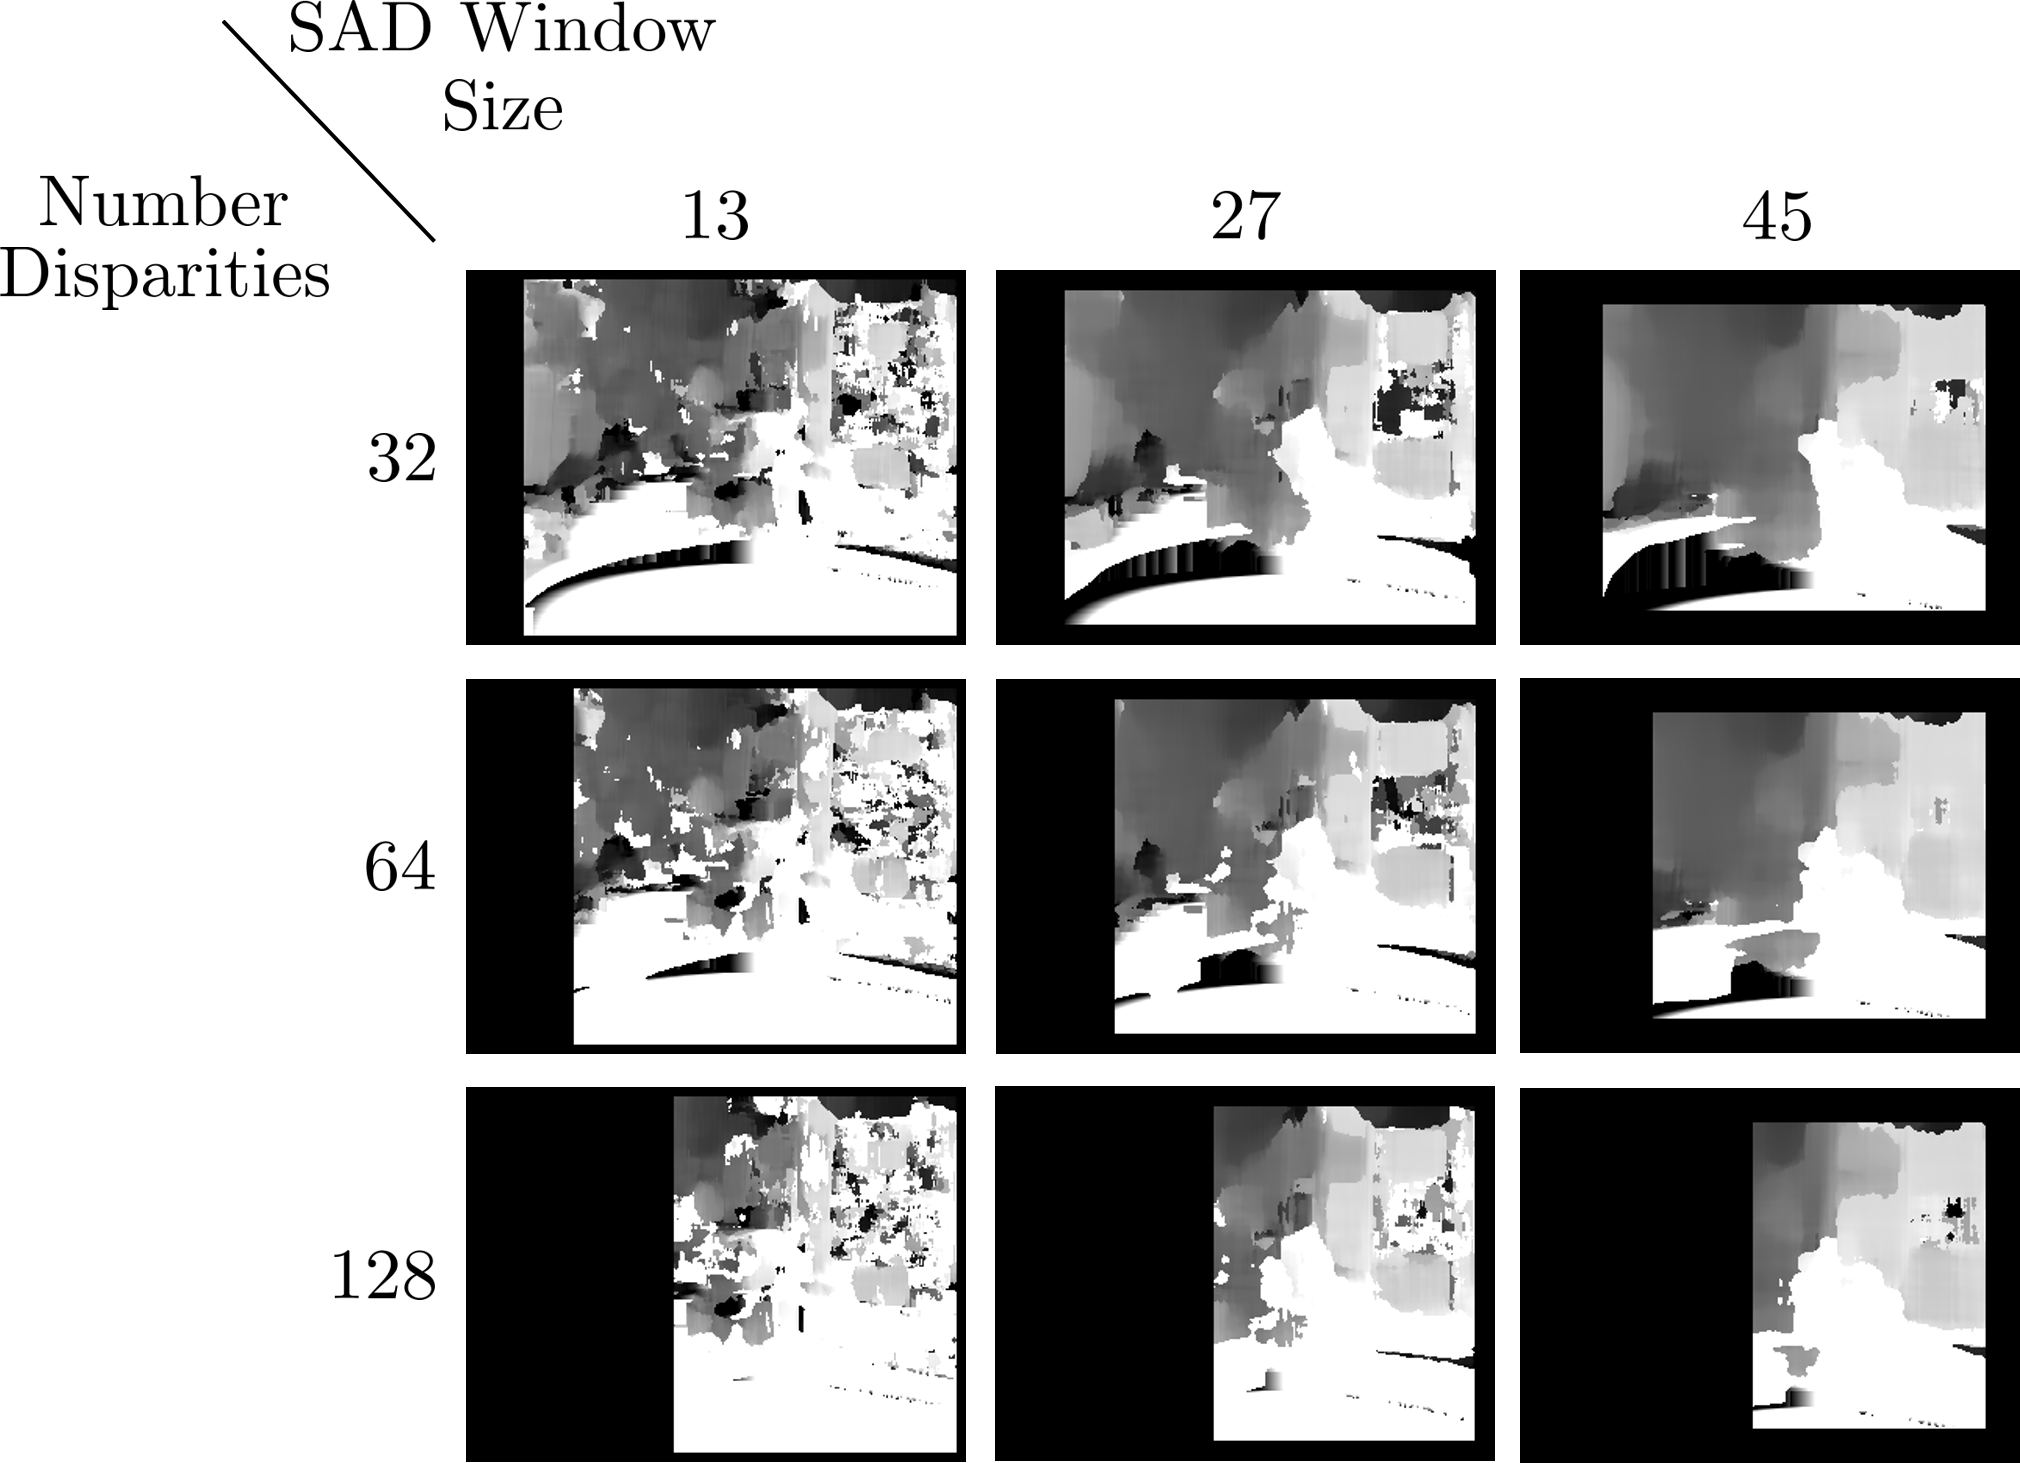
\includegraphics[scale=.28]{chapters/05_experiments/img/disp_sad.png}
	\caption{Left disparity map for changing SAD window sizes and number of disparities. Please refer to figure \ref{fig::324_left_disparity_map} and equation \ref{eq::324_sad} for the theory.}
	\label{fig::52_disp_sad}
\end{figure}
\begin{figure}[h]
	\centering
	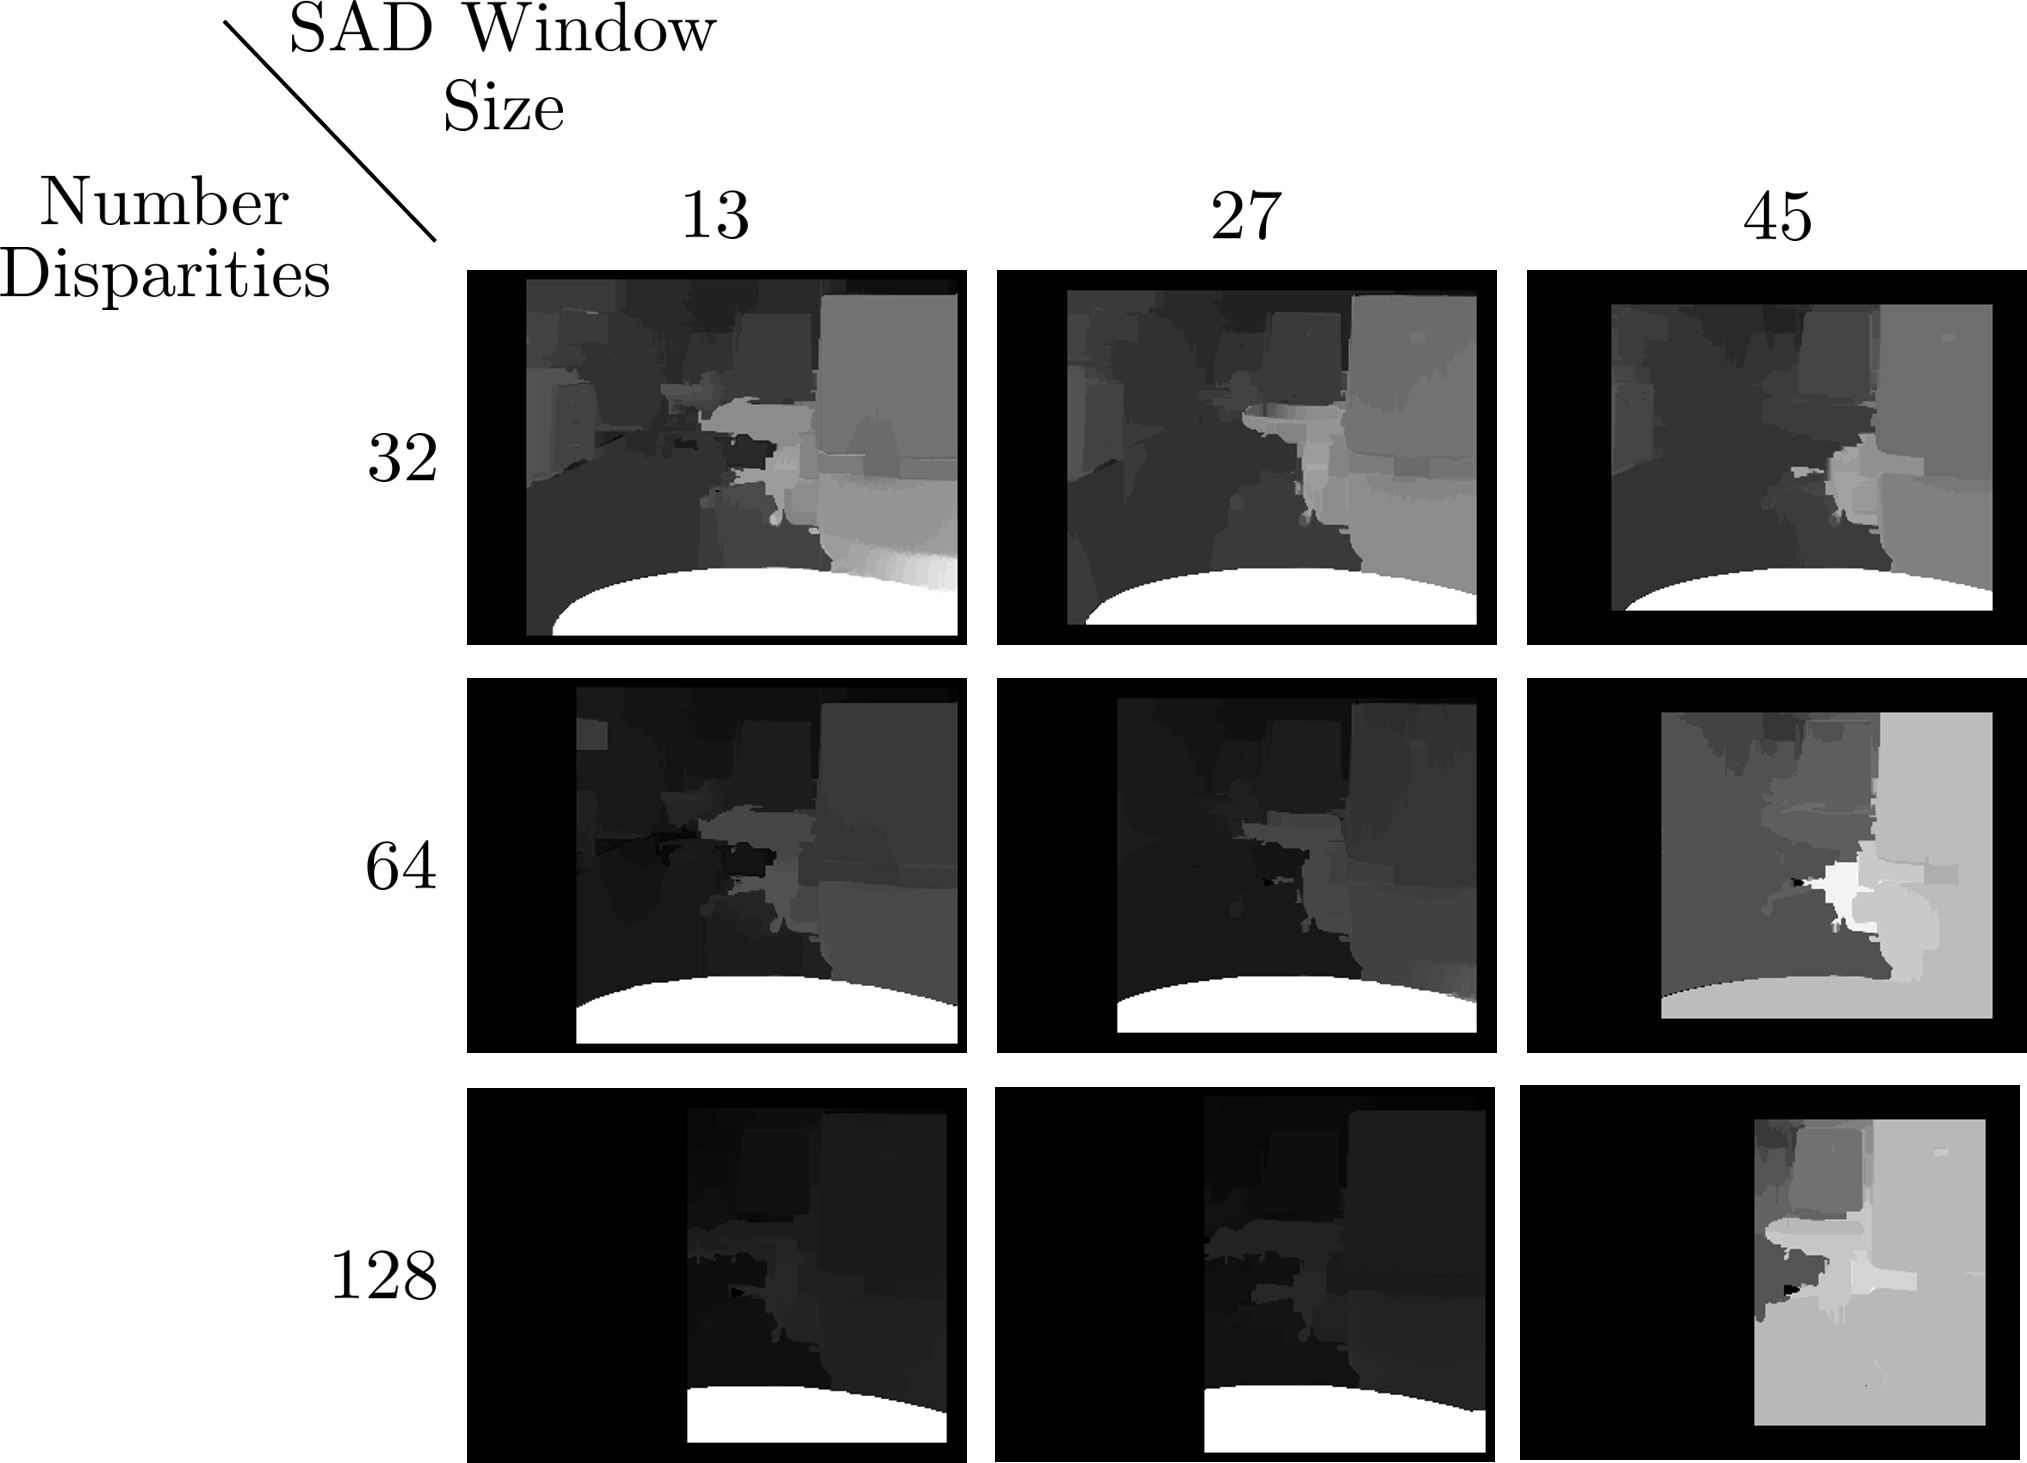
\includegraphics[scale=.28]{chapters/05_experiments/img/disp_sad_wls.png}
	\caption{Confidence weighted least squares disparity for changing SAD windows sizes and number of disparities. Please refer to figure \ref{fig::324_weighted_least_squares_disparity} and equation \ref{eq::324_wls_final} for the theory.}
	\label{fig::52_disp_sad_wls}
\end{figure}
\begin{figure}[h]
	\centering
	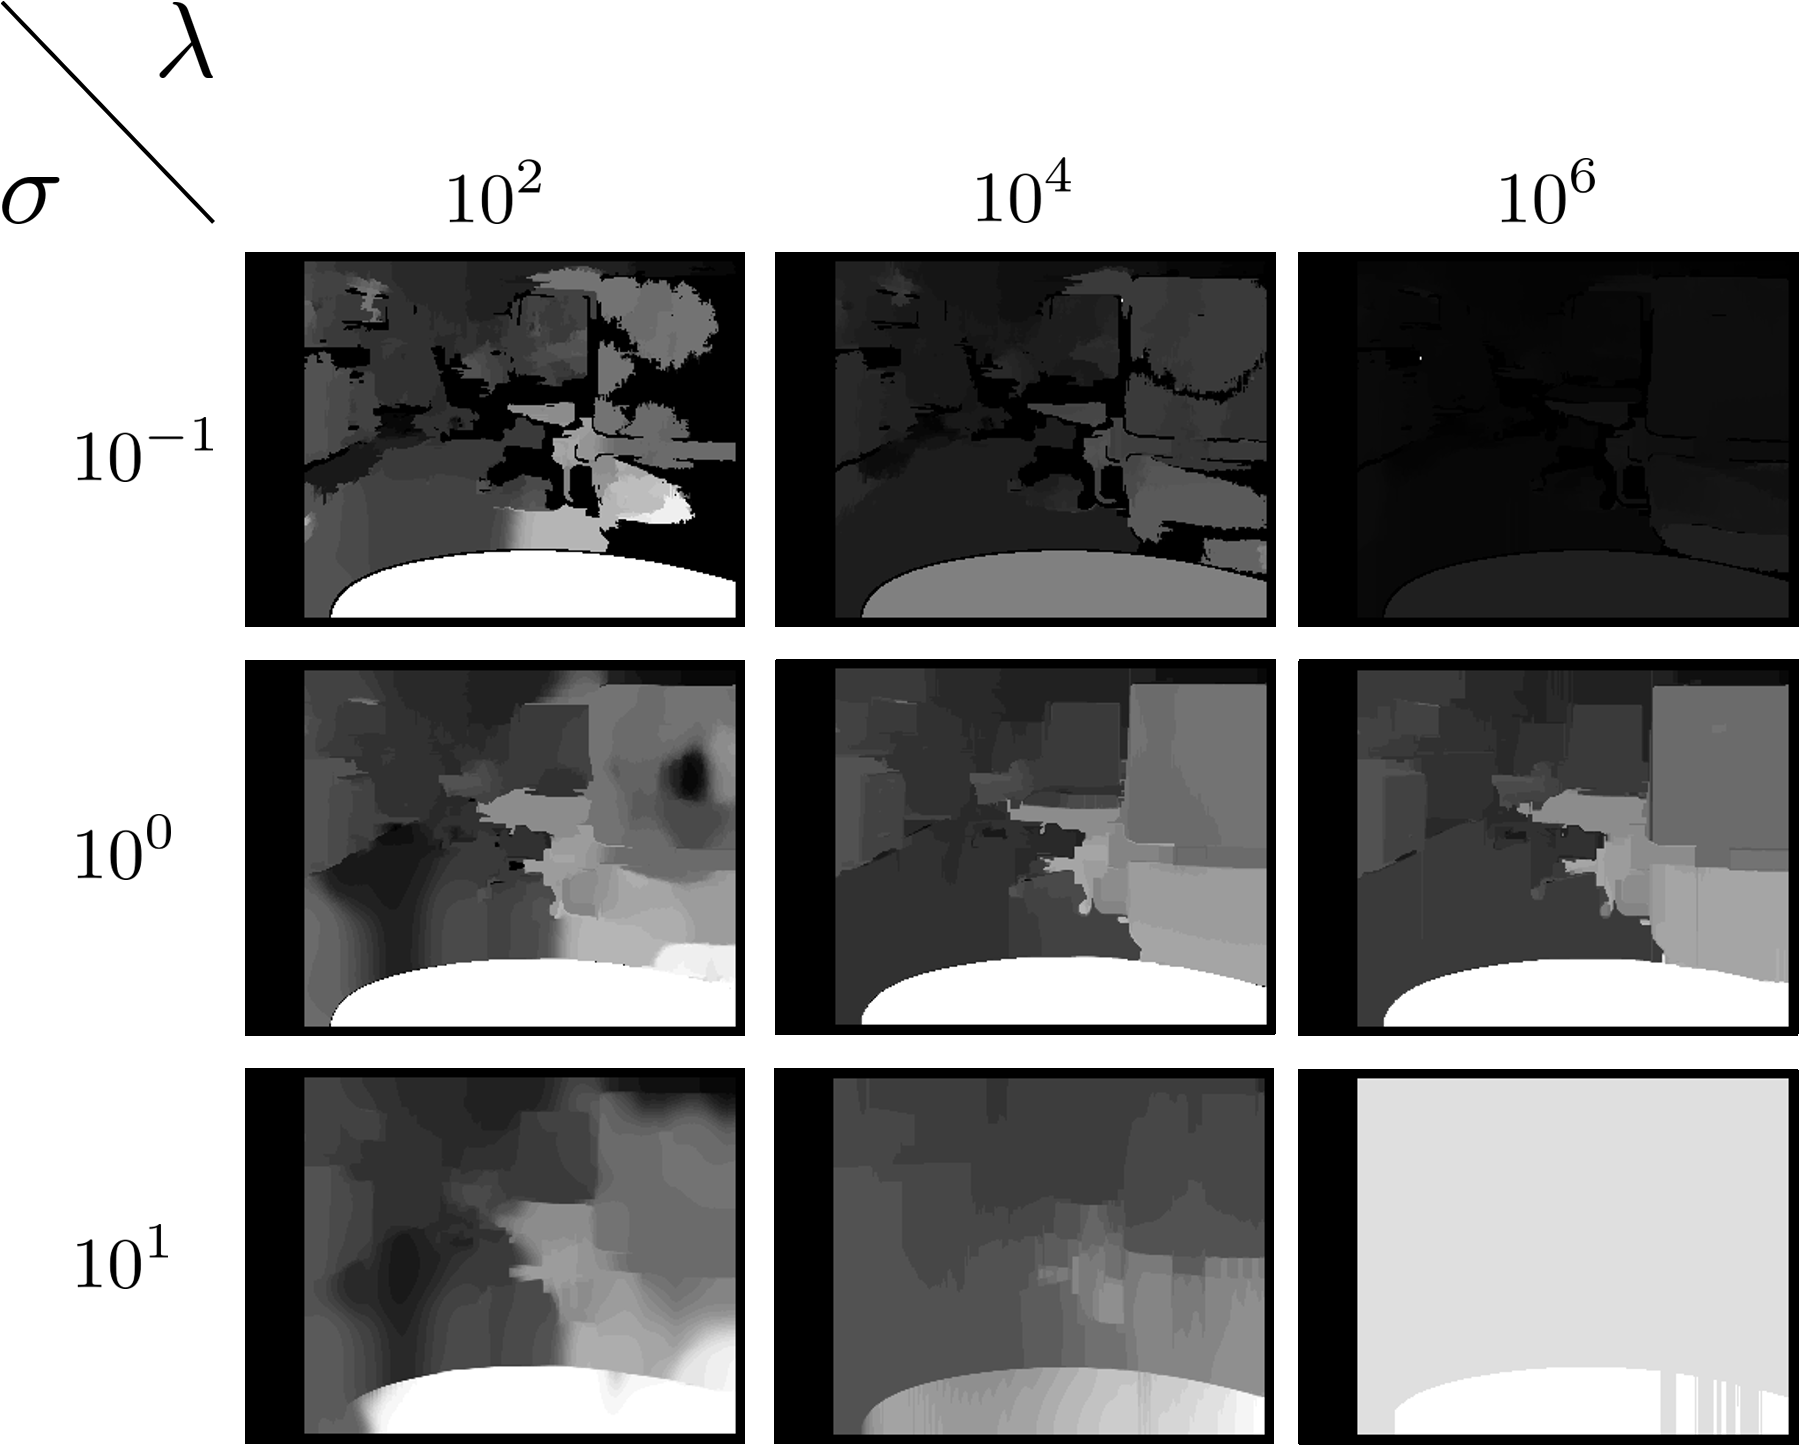
\includegraphics[scale=.28]{chapters/05_experiments/img/sigma_lambda.png}
	\caption{$\sigma$\ref{eq::324_weight} $\lambda$\ref{eq::324_energy_function}}
	\label{fig::52_sigma_lambda}
\end{figure}
\begin{figure}[h]
	\centering
	\subcaptionbox{}%
	[.4\linewidth]{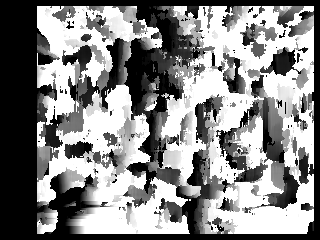
\includegraphics[scale=.3]{chapters/05_experiments/img/disp_no_calib.png}}
	\subcaptionbox{}%
	[.4\linewidth]{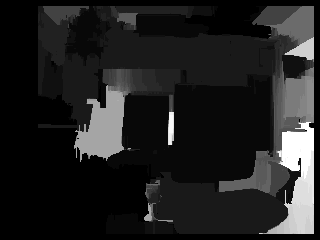
\includegraphics[scale=.3]{chapters/05_experiments/img/wls_no_calib.png}}
	\caption{Left disparity map, and confidence weighted least squares disparity map without rectification.}
	\label{fig::52_no_calib}
\end{figure}